%%%%%%%%%%%%%%%%%%%%%%%%%%%%%%%%%%%%%%%%%%%%%%%%%%%%%%%%%%%%%%%%%%
% The following comments were written in Portuguese, because this 
% template applies only for School of Technology at University 
% of Campinas, Brazil.
%
% Este é um modelo Latex para monografias de Trabalhos de Conclusão 
% de Curso (TCC) na graduação, monografias de Mestrado e Teses de 
% doutorado da Faculdade de Tecnologia (FT) da Universidade 
% Estadual de Campinas (UNICAMP).
%
% Esse modelo e seu respectivo arquivo de classe de documento 
% foram adaptado do modelo de teses e dissertações do 
% Instituto de Computação da UNICAMP.
%
% Autor: André Leon Sampaio Gradvohl, Dr.
% Email:        gradvohl@ft.unicamp.br
% Lattes CV:    http://lattes.cnpq.br/9343261628675642
% ORCID:        0000-0002-6520-9740
% 
% Última versão: 24/Março/2019
%
% Adições/Alterações nesta última versão 
% - Alteração da fonte padrão (times) para fonte libertine, mais 
%   adequada do que a Times New Roman para teses, mas ainda
%   compatível com a times.
% - Adição de comandos para abreviações especiais, e.g., i.e. e
%   p.ex., respectivamente \eg , \ie , \pex
% - Adição do pacote booktabs para tabelas.
% - Ajustes nas referências bibliográficas de acordo com a norma 
%   ABNT NBR 6023 de 14/11/2018.
%%%%%%%%%%%%%%%%%%%%%%%%%%%%%%%%%%%%%%%%%%%%%%%%%%%%%%%%%%%%%%%%%%
%
% Escolha: Portugues ou Ingles ou Espanhol.
% Para a versão final do texto, acrescente a palavra "Final",
% como na segunda linha abaixo da próxima.
%\documentclass[Portugues]{tese-FT}
\documentclass[Portugues,Final]{tese-FT}
%\documentclass[Ingles]{tese-FT}
%\documentclass[Espanhol,Final]{tese-FT}

%Adicione seu arquivo com as referências bibliográficas
\addbibresource{bibliografia.bib}

%O pacote a seguir gera um dummy text. Elimine a linha quando
% for editar seu texto.
%\usepackage{lipsum}
%%%%%%%%%%%%%%%%%%%%%%%%%%%%%
%User packages

\usepackage{soul}
\usepackage{cancel}
\newcommand\tab[1][1cm]{\hspace*{#1}}
\usepackage{amsmath}
\usepackage{minted}
\usepackage{booktabs}
\usepackage{cancel}
\usepackage{enumitem}
\usepackage{subfig}



% Adicione o pacote a seguir, se seu texto tiver uma lista de 
% símbolos. Não confunda com a lista de abreviaturas.
%\usepackage[symbols,nogroupskip,sort=none]{glossaries-extra}

\begin{document}

% Escolha entre autor ou autora:
\autor{Pedro Henrique Neves dos Santos}
%\autora{Nome da Autora}

% Sempre deve haver um título em português:
\titulo{IT306W - Estimação de estado \\ Equação Normal e Tableau Esparso}

% Se a língua for o inglês ou o espanhol defina:
%\title{The Dissertation or Thesis Title in English or Spanish for FT}

% Escolha entre orientador ou orientadora e inclua os títulos:
\orientador{Prof. Dr. Nome do Orientador}
%\orientadora{Profa. Dra. Nome da Orientadora}

% Escolha entre coorientador ou coorientadora, se houver, 
% e inclua os títulos:
%\coorientador{Prof. Dr. Eng. Lic. Nome do Co-Orientador}
%\coorientadora{Prof. Dra. Eng. Lic. Nome da Co-Orientadora}

% Escolha entre uma das quatro opções a seguir (comente as demais):
%\bsi         % para Trabalho de Conclusão de Curso em BSI
%\tads       % para Trabalho de Conclusão de Curso em TADS
%\qualificacaoMestrado  % Para textos de qualificação de mestrado.
%\qualificacaoDoutorado % Para textos de qualificação de doutorado.
\mestrado   % para Dissertação de Mestrado em Tecnologia
%\doutorado  % para Tese de Doutorado em Tecnologia

%Defina a área de concentração. Se for TCC, deixe comentado
\areaConcentracao{Sistemas de Informação e Comunicação}
%\areaConcentracao{Ambiente}
%\areaConcentracao{Ciência dos Materiais}

% Se houve cotutela, defina:
%\cotutela{Universidade Nova de Plutão}

%Defina a data da defesa no formato {Dia}{Mês}{Ano}
\datadadefesa{13}{05}{2020}

% Para a versão final defina:
% Repita o nome do Orientador(a) no primeiro avaliador
%\avaliadorA{Prof. Dr. Nome do Orientador}{FT/UNICAMP}
%\avaliadorB{Profa. Dra. Segunda Avaliadora}{Instituição da segunda avaliadora}
\avaliadorC{Dr. Terceiro Avaliador}{Instituição do terceiro avaliador}
% \avaliadorD{Prof. Dr. Quarto Avaliador}{Instituição do quarto avaliador}
% \avaliadorE{Prof. Dr. Quinto Avaliador}{Instituição do quinto avaliador}
% \avaliadorF{Prof. Dr. Sexto Avaliador}{Instituição do sexto avaliador}
% \avaliadorG{Prof. Dr. Sétimo Avaliador}{Instituição do sétimo avaliador}
% \avaliadorH{Prof. Dr. Oitavo Avaliador}{Instituição do oitavo avaliador}


% Para incluir a ficha catalográfica em PDF na versão final, 
% copie o arquivo PDF, descomente e ajuste a linha a seguir:
%\fichacatalografica{arquivo.pdf}

% Este comando deve ficar aqui:
\paginasiniciais
% Sempre deve haver um resumo em português:
\begin{resumo}

%Primeiro trabalho apresentado \`a disciplina IT306.\\\\\
Neste quarto trabalho, será abordado os Estimadores de Estado, usando Equação Normal e Tableau Esparso. \\
Todos os códigos podem ser encontrados em \\
\href{https://github.com/phneves/ElectricPowerSystemsAnalysisTools}{https://github.com/phneves/ElectricPowerSystemsAnalysisTools}



\end{resumo}


% A lista de símbolos é opcional. Não confunda a lisa de símbolos
% com a lista de abreviaturas.
%\prefacesection{Lista de Símbolos}

% Coloque o símbolo na primeira coluna e a 
% descrição na segunda coluna. Use descrições
% rápidas.

\begin{table}[!ht]
  \begin{tabular}{p{3cm}l}
	$NB$        & N\'umero de Barras \\
	$k$       & Inteiro entre 1 e $NB$\\
	$m$        & N\'umero de Barras \\
	$\in$       & Inteiro entre 1 e $NB$\\
	$\kappa$        & Conjunto formado pela barra $k$ e todas as barras $m$ conectadas ela \\
	$G_{km}$       & Inteiro entre 1 e $NB$\\
	$B_{km}$        & N\'umero de Barras \\
	$k$       & Inteiro entre 1 e $NB$\\
	
	$c$       & Descrição do símbolo $c$ 
  \end{tabular}
\end{table}

% A lista de abreviações e siglas vem a seguir.
% Dê uma olhada no pacote nomencl para ver os comandos para 
% adicionar abreviações e siglas no texto.
\renewcommand{\nomname}{Lista de Abreviações e Siglas}
\printnomenclature[3cm]


% O sumário vem aqui:
\tableofcontents
\fimdaspaginasiniciais


% O corpo da dissertação ou tese começa aqui:
%
% O comando a seguir inclui o arquivo introducao.tex
% que contém o capítulo de Introdução. 
% Detalhe: não precisa incluir a extensão .tex
%\include{introducao}


\chapter{Introdu\c{c}\~ao e teoria}
%Estimação de estados 
%exemplo na pagina 16 do slide semana 7 
%Abordar método dos mínimos quadrados
%livro do monticelli - pag 268 - 




%\section{Motiva\c{c}\~ao}

% DIZER ALGO SOBRE COMO SERA O SISTEMA, COM BARRAS E CONEXOES E QUE FICA COMPLEXO SEM ANALISE DE FLUXO DE CARGA Mas como \'e possivel garantir o planejamento e opera\c{c}\~ao sistema de grandes propor\c{c}\~oes como esse? Para isso, \'e preciso saber o estado atual do sistema. Por\'em, n\~ao \'e vi\'avel medir todos os pontos de interesse. Isso seria custoso e tomaria muito tempo. 


%Para  como um todo \'e necessario que tenhamos ferramentas que nos ajudem a estimar o estado da rede 

%\section{Introdução à Teoria}
A ferramenta de an\'alise de sistemas de energia el\'etrica aqui discutida ser\'a a Estimação de Estado. Essa an\'alise nos fornecer\'a um metodo de obter o estado mais provável do sistema (ou de parte dele) a partir de medidas realizadas e a partir do modelo (circuito equivalente) da rede. \cite{monticelli}.
\section{Modelagem}
\label{SectionIntro}
%texto que explica como funciona
Para estimar o estado, será utilizado um conjunto de medidas que há disponível. Todas as redes de energia elétrica são constantemente monitoradas e, como toda medida, há uma incenteza atrelada, podendo ser erros aceitáveis e inaceitáveis (erros grosseiros).\\
É necessário que haja número de medidas em quantidade suficiente, para minimizar a influência dos erros grosseiros. Aliás, na hipótese de haver redundância no conjunto de medidas, é possível tratar erros nas medidas, já que pode-se lançar mão de ferramentas estatísticas.\\
Frequentemente, os valores calculados com o estado estimado, são mais confiáveis que o conjunto de medidas. \\
O modelo da rede e composto basicamente pelos circuitos equivalentes das linhas, transformadores, reguladores de tensão e por um gerador que proverá a referência angular da rede. Dispositivos de chaveamento e geradores distribuídos também podem ser modelados.\\
A topologia da rede e determinada pelo Configurador Topológico, que deve ser executado a cada alteração na topologia da rede.\cite{castro}

%formulas usadas no código
\section{Formula\c{c}\~ao do problema b\'asico}
\subsection{Mínimos Quadrados Ponderado}
Será utilizado modelos que descrevem as medições e suas relações, como em \ref{EQ_Modelo}

\begin{equation}
    z = \left[ 
    \begin{matrix} 
        z_1 \\
        z_2 \\
        \vdots \\
        z_m
    \end{matrix} \right]=\left[ 
    \begin{matrix} 
        h_1(x_1,x_2,...,x_n) \\
        h_2(x_1,x_2,...,x_n) \\
        \vdots \\
        h_m(x_1,x_2,...,x_n)
    \end{matrix} \right]+\left[ 
    \begin{matrix} 
        e_1 \\
        e_2 \\
        \vdots \\
        e_m
    \end{matrix} \right] = h(x) + e
    \label{EQ_Modelo}
\end{equation}
Onde $h_i(x)$ é a função que correlaciona a i-ésima medição com o vetor de estado, $x^t = [x_1, x_2,\hdots, x_n ]$ é o vetor de estado que contém as n variáveis de estado e $e^t = [e_1, e_2,\hdots, e_m ]$ corresponde ao vetor de erros do processo de medição.\\
Os elementos de $e$ possuem média nula, $E\{e_i e_i\} = 0$, e $Cov(e) = E[e.e^t] = R_z = diag\{\sigma_1^2, \sigma_2^2, \hdots, \sigma_m^2\}$. A variância $\sigma_i^2$ é calculada de acordo com a precisão da medição.\\
No método dos mínimos quadrados ponderados a função \ref{EQ_Jacobiana} deve ser minimizada. O inverso do desvio padrão é usado na ponderação das medidas. \cite{castro}
\begin{equation}
    J(x) = \sum_{i=1}^{m} \frac{(z_i - h_i(x))^2}{\sigma_i^2} = [z-h(x)]'R_z^-1[z-h(x)]
    \label{EQ_Jacobiana}
\end{equation}
\subsection{Equação normal}
\label{SectionFormula}
Ao minimizar a equação \ref{EQ_Jacobiana}, é necessário derivá-la e igualar a zero. Como resultado, o estado estimado é obtido iterativamente com método dos minimos quadrados ponderados, conforme a equação \ref{WLS_G}.
\begin{equation}
    G(x^\nu). \Delta x^\nu = H'(x^\nu).R_z^-1 [z-H(x^\nu)]
    \label{WLS_G}
\end{equation}
E,
\begin{equation}
    x^{\nu+1} = x^\nu + \Delta x^\nu
\end{equation}
A matriz Hessiana $G(x)$, chamada de matriz Ganho, é definida como em \ref{G}
\begin{equation}
    G(x) = H'(x)R_z^{-1}H(x)
    \label{G}
\end{equation}
O uso da matriz $G$, de ganhos, é conhecido como solução via equação normal e esta solução apresenta boa convergênca. Em alguns casos, porém, a solução da equação \ref{WLS_G} pode apresentar divergência (não será abordado neste trabalho).\\
A formação da matriz $H$, descrita em \ref{G}, é dada por \ref{H}.
\begin{figure}[!htb]
\caption{Formulação da matriz $H$}
 \centering % para centralizarmos a figura
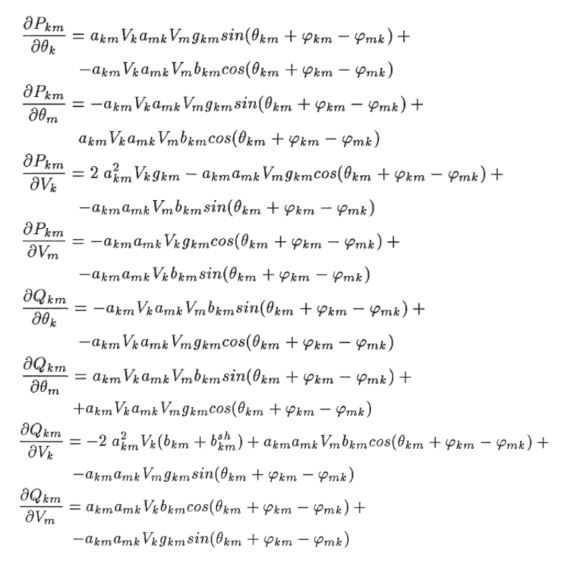
\includegraphics[width=12cm]{figuras/H.JPG}
\label{H}
\end{figure}
\subsection{Tableau Esparso}
Para evitar trabalhar com o produto de H (matriz G), como em \ref{G}, pode-se reescrever o problema como minimização com restrições, como em \ref{EQ_minJ} e \ref{EQ_minJ2}
\begin{equation}
    minJ(x) = \frac{1}{2}[z-h(x)]R_z^{-1} [z-h(x)]
    \label{EQ_minJ}
\end{equation}
\begin{equation}
    minJ(x) = \frac{1}{2}r'R_z^{-1}r
    \label{EQ_minJ2}
\end{equation}
Sujeito a $r = z-h(x)$. 
Para resolver este problema, deve-se usar multiplicadores de Lagrange. A solução pode ser obtida iterativamente a partir de \ref{EQ_Tableau}.
\begin{equation}
    \left[ 
    \begin{matrix} 
        R_z & H(x^k) \\
        H'(x^k) & 0
    \end{matrix} \right] \left( 
    \begin{matrix} 
        \lambda^k \\
        \Delta x^k
    \end{matrix} \right) = \left[ 
    \begin{matrix} 
        z-h(x^k) \\
        0
    \end{matrix} \right]= \left[ 
    \begin{matrix} 
        \Delta z(x^k) \\
        0
    \end{matrix} \right]
    \label{EQ_Tableau}
\end{equation}
Neste processo, há a matriz $H$ e não a matriz $G$, o que melhora o condicionamento da matriz a ser fatorada. \cite{castro}. 

%%%%%%%%%%%%%%%%%%%
\section{Algoritmo implementado}
Basicamente, tem-se 4 etapas do processo de estimação de estado \cite{Mohamad}. 
\begin{enumerate}
    \item Processamento da topologia. Todas as informações de representação da topologia são tratadas.
    \item Analise de observabilidade. A partir do modelo barra-ramo obtido na primeira etapa, verifica-se se é possivel determinar as tensões e angulos em todas as barras, considerando as medidas disponíveis.
    \item Estimação de estado. A partir da topologia, dos parâmetros e dos conjuntos de medidas disponíveis, o Estimador de Estado determina a estimação que melhor representa o sistema
    \item Processamento de erros grosseiros. A presença de medidas analógicas com possibilidade de erros grosseiros afasta a solução verdadeira do estimador de estados. Se uma medida é identificada dessa forma, ela deve ser retirada da solução. 
    
\end{enumerate}



\chapter{Estudos de caso}
\label{SectionEstudosDeCaso}
Neste capítulo, será estudado a rede de 14 barras do IEEE que pode ser encontrado em \\ \href{http://labs.ece.uw.edu/pstca/pf14/pg_tca14bus.htm}{http://labs.ece.uw.edu/pstca/pf14/pg\_tca14bus.htm}
\section{Rede de 14 barras IEEE}
\label{SectionRedePequena}
Considere a rede de 14 barras na figura \ref{FigRede4barrasLinearizado}.\\
\begin{figure}[!htb]
\caption{Rede de 14 barras IEEE}
 \centering % para centralizarmos a figura
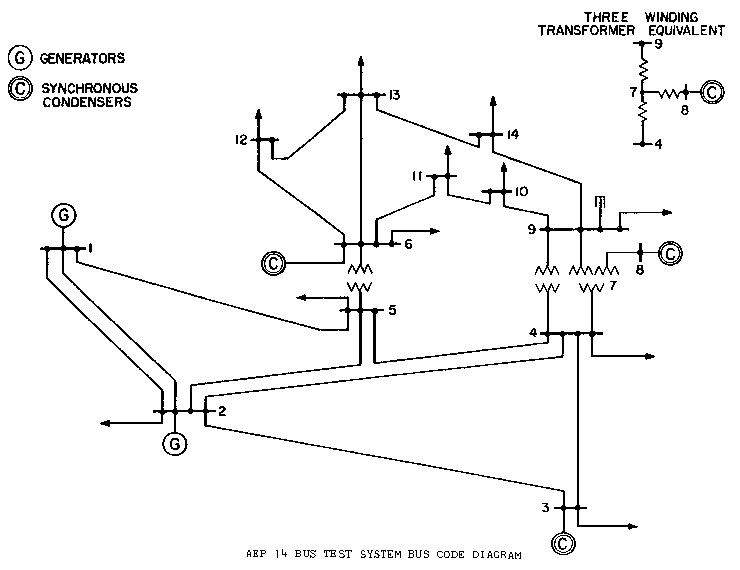
\includegraphics[width=12cm]{figuras/14bus.jpg}
\label{FigRede4barrasLinearizado}
\end{figure}
Neste exercício, será resolvido as tensões e angulos de todas as barras desse sistema, utilizando dados de medições disponíveis na rede. 
\subsection{Dados do Problema}
\label{SectionDados}
Medições do problema \ref{SectionRedePequena}. São dados obtidos da rede que serão usados para estimar o estado do sistema.
\begin{minted}[mathescape, style = autumn,
    frame = single, fontsize=\footnotesize]{matlab}
%         |Msnt |Type | Value | From | To | Rii | 
zdata14   = [ %---- Voltage Magnitude ------------%
            1     1    1.06     1       0   9e-4;
            %-----------------------------------%
            %---- Real Power Injection ---------%
            2     2    0.1830   2       0   1e-4;
            3     2   -0.9420   3       0   1e-4; 
            4     2    0.00     7       0   1e-4;
            5     2    0.00     8       0   1e-4; 
            6     2   -0.0900  10       0   1e-4;
            7     2   -0.0350  11       0   1e-4;
            8     2   -0.0610  12       0   1e-4; 
            9     2   -0.1490  14       0   1e-4;
           %------------------------------------%
           %---- Reative Power Injection -------%
           10     3    0.3523   2       0   1e-4;
           11     3    0.0876   3       0   1e-4; 
           12     3    0.00     7       0   1e-4;
           13     3    0.2103   8       0   1e-4; 
           14     3   -0.0580  10       0   1e-4;
           15     3   -0.0180  11       0   1e-4;
           16     3   -0.0160  12       0   1e-4; 
           17     3   -0.0500  14       0   1e-4;
           %------------------------------------%
           %------ Real Power Flow ------------- %
           18     4    1.5708   1       2   64e-6;
           19     4    0.7340   2       3   64e-6;
           20     4   -0.5427   4       2   64e-6;
           21     4    0.2707   4       7   64e-6;
           22     4    0.1546   4       9   64e-6;
           23     4   -0.4081   5       2   64e-6;
           24     4    0.6006   5       4   64e-6;
           25     4    0.4589   5       6   64e-6;
           26     4    0.1834   6      13   64e-6;
           27     4    0.2707   7       9   64e-6;
           28     4   -0.0816  11       6   64e-6;
           29     4    0.0188  12      13   64e-6;
           %------------------------------------%
           %------ Real Power Flow ------------- %
           30     5   -0.1748   1       2   64e-6;
           31     5    0.0594   2       3   64e-6;
           32     5    0.0213   4       2   64e-6;
           33     5   -0.1540   4       7   64e-6;
           34     5   -0.0264   4       9   64e-6;
           35     5   -0.0193   5       2   64e-6;
           36     5   -0.1006   5       4   64e-6;
           37     5   -0.2084   5       6   64e-6;
           38     5    0.0998   6      13   64e-6;
           39     5    0.1480   7       9   64e-6;
           40     5   -0.0864  11       6   64e-6;
           41     5    0.0141  12      13   64e-6;];
           %--------------------------------------%
\end{minted}

%%%%%%%%%%%%%%%%%%%%%%%%%%%%%%%%%%%%%%%%%%%%%%%
Dados das barras do problema \ref{SectionRedePequena}
\begin{minted}[mathescape, style = autumn,
    frame = single, fontsize=\footnotesize]{matlab}
% |Bus | Type | Vsp | theta | PGi | QGi | PLi | QLi |  Qmin | Qmax |
busdata14 = 
[ 1     1    1.060   0       0     0     0     0       0       0;
  2     2    1.045   0      40   42.4  21.7   12.7    -40     50;
 3     2    1.010   0       0   23.4  94.2   19.0     0      40;
 4     3    1.0     0       0     0   47.8   -3.9     0       0;
 5     3    1.0     0       0     0    7.6    1.6     0       0;
 6     2    1.070   0       0   12.2  11.2    7.5    -6      24;
 7     3    1.0     0       0     0    0.0    0.0     0       0;
 8     2    1.090   0       0   17.4   0.0    0.0    -6      24;
 9     3    1.0     0       0     0   29.5   16.6     0       0;
 10    3    1.0     0       0     0    9.0    5.8     0       0;
 11    3    1.0     0       0     0    3.5    1.8     0       0;
 12    3    1.0     0       0     0    6.1    1.6     0       0;
 13    3    1.0     0       0     0   13.5    5.8     0       0;
 14    3    1.0     0       0     0   14.9    5.0     0       0;];
\end{minted}
Dados dos ramos do problema \ref{SectionRedePequena}
\begin{minted}[mathescape, style = autumn,
    frame = single, fontsize=\footnotesize]{matlab}
%         |  From |  To   |   R     |   X     |     B/2  |  X'mer  |
%         |  Bus  | Bus   |  pu     |  pu     |     pu   | TAP (a) |
linedata14 =[1      2       0.01938   0.05917    0.0264         1
             1      5       0.05403   0.22304    0.0246         1
             2      3       0.04699   0.19797    0.0219         1
             2      4       0.05811   0.17632    0.0170         1
             2      5       0.05695   0.17388    0.0173         1
             3      4       0.06701   0.17103    0.0064         1
             4      5       0.01335   0.04211    0.0            1
             4      7       0.0       0.20912    0.0        0.978
             4      9       0.0       0.55618    0.0        0.969
             5      6       0.0       0.25202    0.0        0.932
             6     11       0.09498   0.19890    0.0            1
             6     12       0.12291   0.25581    0.0            1
             6     13       0.06615   0.13027    0.0            1
             7      8       0.0       0.17615    0.0            1
             7      9       0.0       0.11001    0.0            1
             9     10       0.03181   0.08450    0.0            1
             9     14       0.12711   0.27038    0.0            1
            10     11       0.08205   0.19207    0.0            1
            12     13       0.22092   0.19988    0.0            1
            13     14       0.17093   0.34802    0.0            1 ];
\end{minted}

\section{Resultado do Estimador de Estados}
\label{SectionResultados}
Os resultados das duas soluções convergiram para esse problema. Nota-se que o tempo computacional utilizando Tableau Esparso é menor, embora a comparação tenha apenas efeito didático já que o processador não é dedicado e pode variar o tempo de solução.

\subsection{Equação Normal}
Aqui, a matriz $G$ foi calculada como em \ref{G}. O código está na seção \ref{SectionEqNormal}
\begin{minted}[mathescape, style = autumn,
    frame = single, fontsize=\footnotesize]{matlab}
    
-------- State Estimation ------------------
--------------------------
| Bus |    V   |  Angle  | 
| No  |   pu   |  Degree | 
--------------------------
   1    1.0068     0.0000
   2    0.9899    -5.5265
   3    0.9518   -14.2039
   4    0.9579   -11.4146
   5    0.9615    -9.7583
   6    1.0185   -16.0798
   7    0.9919   -14.7510
   8    1.0287   -14.7500
   9    0.9763   -16.5125
  10    0.9758   -16.7476
  11    0.9932   -16.5397
  12    1.0009   -17.0203
  13    0.9940   -17.0583
  14    0.9647   -17.8967
---------------------------------------------
Tempo computacional =  0.0834 segundos.
\end{minted}
\subsection{Tableau Esparso}
Aqui, a matriz $G$ não foi calculada. O calculo foi feito como em \ref{EQ_Tableau}. O código está na seção \ref{SectionTableau}
\begin{minted}[mathescape, style = autumn,
    frame = single, fontsize=\footnotesize]{matlab}
    
-------- State Estimation ------------------
-------- Tableau Sparse   ------------------
--------------------------
| Bus |    V   |  Angle  | 
| No  |   pu   |  Degree | 
--------------------------
   1    1.0068     0.0000
   2    0.9899    -5.5265
   3    0.9518   -14.2039
   4    0.9579   -11.4146
   5    0.9615    -9.7583
   6    1.0185   -16.0798
   7    0.9919   -14.7510
   8    1.0287   -14.7500
   9    0.9763   -16.5125
  10    0.9758   -16.7476
  11    0.9932   -16.5397
  12    1.0009   -17.0203
  13    0.9940   -17.0583
  14    0.9647   -17.8967
---------------------------------------------
Tempo computacional =  0.0469 segundos.
\end{minted}

\chapter{C\'odigo comentado}
\label{SectionCodigo}

Os códigos fonte desse trabalho bem como histórico de modificação, podem ser encontrados no endereço: \textit{\href{https://github.com/phneves/ElectricPowerSystemsAnalysisTools}{https://github.com/phneves/ElectricPowerSystemsAnalysisTools}}.\\
Entrada de dados do estimador de estados.
\begin{minted}[mathescape, style = autumn,
    frame = single, fontsize=\footnotesize]{matlab}
num = 14; 
ybus = ybusppg(num); 
zdata = zdatas(num); %pneves: Get Measurement data
bpq = bbusppg(num); % Get B data
nbus = max(max(zdata(:,4)),max(zdata(:,5))); % Get number of buses
type = zdata(:,2);
z = zdata(:,3); % Measuement values
fbus = zdata(:,4); % From bus
tbus = zdata(:,5); % To bus
Ri = diag(zdata(:,6)); % Measurement Error
V = ones(nbus,1); % Initialize the bus voltages
del = zeros(nbus,1); % Initialize the bus angles
E = [del(2:end); V];   % State Vector
G = real(ybus);
B = imag(ybus);
\end{minted}

\begin{minted}[mathescape, style = autumn,
    frame = single, fontsize=\footnotesize]{matlab}
vi = find(type == 1); % Index of voltage magnitude measurements
ppi = find(type == 2); % Index of real power injection measurements
qi = find(type == 3); % Index of reactive power injection measurements
pf = find(type == 4); % Index of real powerflow measurements
qf = find(type == 5); % Index of reactive powerflow measurements
\end{minted}
Calcula o número de medidas disponíveis.
\begin{minted}[mathescape, style = autumn,
    frame = single, fontsize=\footnotesize]{matlab}
%pneves
nvi = length(vi); % Number of Voltage measurements
npi = length(ppi); % Number of Real Power Injection measurements
nqi = length(qi); % Number of Reactive Power Injection measurements
npf = length(pf); % Number of Real Power Flow measurements
nqf = length(qf); % Number of Reactive Power Flow measurements
iter = 1;
tol = 5;
\end{minted}
%%%%%%%%%%%%%%%%%%%%%%%%%%%%%%%%%%%%%%%%%%%%%%%%%%%%%%%%%%%%%%%%%%%%%%%%%%%%%%%%%%%%%%%%%%%%%%%%
Itera-se comparando com a tolerância desejada. 
\begin{minted}[mathescape, style = autumn,
    frame = single, fontsize=\footnotesize]{matlab}
while(tol > 1e-4)
    %Measurement Function, h 
    h1 = V(fbus(vi),1);
    h2 = zeros(npi,1);
    h3 = zeros(nqi,1);
    h4 = zeros(npf,1);
    h5 = zeros(nqf,1);
\end{minted}
%%%%%%%%%%%%%%%%%%%%%%%%%%%%%%%%%%%%%%%%%%%%%%%%%%%%%%%%%%%%%%%%%%%%%%%%%%%%%%%%%%%%%%%%%%%%%%%%

\begin{minted}[mathescape, style = autumn,
    frame = single, fontsize=\footnotesize]{matlab}

    for i = 1:npi
        m = fbus(ppi(i));
        for k = 1:nbus
            h2(i) = h2(i) + V(m)*V(k)*(G(m,k)*cos(del(m)-del(k)) + ...
                B(m,k)*sin(del(m)-del(k)));
        end
    end
    
    for i = 1:nqi
        m = fbus(qi(i));
        for k = 1:nbus
            h3(i) = h3(i) + V(m)*V(k)*(G(m,k)*sin(del(m)-del(k)) - ...
                B(m,k)*cos(del(m)-del(k)));
        end
    end
    
    for i = 1:npf
        m = fbus(pf(i));
        n = tbus(pf(i));
        h4(i) = -V(m)^2*G(m,n) - V(m)*V(n)*(-G(m,n)*cos(del(m)-del(n))
            - B(m,n)*sin(del(m)-del(n)));
    end
    
    for i = 1:nqf
        m = fbus(qf(i));
        n = tbus(qf(i));
        h5(i) = -V(m)^2*(-B(m,n)+bpq(m,n)) 
            - V(m)*V(n)*(-G(m,n)*sin(del(m)-del(n))
            + B(m,n)*cos(del(m)-del(n)));
    end
    
    h = [h1; h2; h3; h4; h5];
    
    %pneves: Residue
    r = z - h;
\end{minted}
%%%%%%%%%%%%%%%%%%%%%%%%%%%%%%%%%%%%%%%%%%%%%%%%%%%%%%%%%%%%%%%%%%%%%%%%%%%%%%%%%%%%%%%%%%%%%%%%
Monta-se a matriz Jacobiana seguindo \ref{H}.\\
$H_{11}$ Derivada de $V$ com respeito a $\theta$.
\begin{minted}[mathescape, style = autumn,
    frame = single, fontsize=\footnotesize]{matlab}

    H11 = zeros(nvi,nbus-1);

\end{minted}
%%%%%%%%%%%%%%%%%%%%%%%%%%%%%%%%%%%%%%%%%%%%%%%%%%%%%%%%%%%%%%%%%%%%%%%%%%%%%%%%%%%%%%%%%%%%%%%%
$H_{12}$ Derivada de $V$ com respeito a $V$.
\begin{minted}[mathescape, style = autumn,
    frame = single, fontsize=\footnotesize]{matlab}
    H12 = zeros(nvi,nbus);
    for k = 1:nvi
        for n = 1:nbus
            if n == k
                H12(k,n) = 1;
            end
        end
    end
\end{minted}
%%%%%%%%%%%%%%%%%%%%%%%%%%%%%%%%%%%%%%%%%%%%%%%%%%%%%%%%%%%%%%%%%%%%%%%%%%%%%%%%%%%%%%%%%%%%%%%%
$H_{21}$ Derivada de $P$ com respeito a $\theta$.
\begin{minted}[mathescape, style = autumn,
    frame = single, fontsize=\footnotesize]{matlab}
    H21 = zeros(npi,nbus-1);
    for i = 1:npi
        m = fbus(ppi(i));
        for k = 1:(nbus-1)
            if k+1 == m
                for n = 1:nbus
                    H21(i,k) = H21(i,k) + ...
                        V(m)* V(n)*(-G(m,n)*sin(del(m)-del(n)) + ...
                        B(m,n)*cos(del(m)-del(n)));
                end
                H21(i,k) = H21(i,k) - V(m)^2*B(m,m);
            else
                H21(i,k) = V(m)* V(k+1)*(G(m,k+1)*sin(del(m)-del(k+1)) 
                - B(m,k+1)*cos(del(m)-del(k+1)));
            end
        end
    end
\end{minted}
%%%%%%%%%%%%%%%%%%%%%%%%%%%%%%%%%%%%%%%%%%%%%%%%%%%%%%%%%%%%%%%%%%%%%%%%%%%%%%%%%%%%%%%%%%%%%%%%
$H_{22}$ Derivada de $P$ com respeito a $V$.
\begin{minted}[mathescape, style = autumn,
    frame = single, fontsize=\footnotesize]{matlab}    
    H22 = zeros(npi,nbus);
    for i = 1:npi
        m = fbus(ppi(i));
        for k = 1:(nbus)
            if k == m
                for n = 1:nbus
                    H22(i,k) = H22(i,k) + ...
                    V(n)*(G(m,n)*cos(del(m)-del(n)) + ...
                    B(m,n)*sin(del(m)-del(n)));
                end
                H22(i,k) = H22(i,k) + V(m)*G(m,m);
            else
                H22(i,k) = V(m)*(G(m,k)*cos(del(m)-del(k)) + ...
                B(m,k)*sin(del(m)-del(k)));
            end
        end
    end
\end{minted}
%%%%%%%%%%%%%%%%%%%%%%%%%%%%%%%%%%%%%%%%%%%%%%%%%%%%%%%%%%%%%%%%%%%%%%%%%%%%%%%%%%%%%%%%%%%%%%%%
$H_{31}$ Derivada de $Q$ com respeito a $\theta$.
\begin{minted}[mathescape, style = autumn,
    frame = single, fontsize=\footnotesize]{matlab}    
    H31 = zeros(nqi,nbus-1);
    for i = 1:nqi
        m = fbus(qi(i));
        for k = 1:(nbus-1)
            if k+1 == m
                for n = 1:nbus
                    H31(i,k) = H31(i,k) + ...
                    V(m)* V(n)*(G(m,n)*cos(del(m)-del(n)) + ...
                    B(m,n)*sin(del(m)-del(n)));
                end
                H31(i,k) = H31(i,k) - V(m)^2*G(m,m);
            else
               H31(i,k) = V(m)* V(k+1)*(-G(m,k+1)*cos(del(m)-del(k+1)) 
               - B(m,k+1)*sin(del(m)-del(k+1)));
            end
        end
    end
\end{minted}
%%%%%%%%%%%%%%%%%%%%%%%%%%%%%%%%%%%%%%%%%%%%%%%%%%%%%%%%%%%%%%%%%%%%%%%%%%%%%%%%%%%%%%%%%%%%%%%%
$H_{32}$ Derivada de $Q$ com respeito a $V$.
\begin{minted}[mathescape, style = autumn,
    frame = single, fontsize=\footnotesize]{matlab}    
    H32 = zeros(nqi,nbus);
    for i = 1:nqi
        m = fbus(qi(i));
        for k = 1:(nbus)
            if k == m
                for n = 1:nbus
                    H32(i,k) = H32(i,k) + ...
                    V(n)*(G(m,n)*sin(del(m)-del(n)) - ...
                    B(m,n)*cos(del(m)-del(n)));
                end
                H32(i,k) = H32(i,k) - V(m)*B(m,m);
            else
               H32(i,k) = V(m)*(G(m,k)*sin(del(m)-del(k)) 
               - B(m,k)*cos(del(m)-del(k)));
            end
        end
    end
\end{minted}
%%%%%%%%%%%%%%%%%%%%%%%%%%%%%%%%%%%%%%%%%%%%%%%%%%%%%%%%%%%%%%%%%%%%%%%%%%%%%%%%%%%%%%%%%%%%%%%%
$H_{41}$ Derivada de $P$ com respeito a $\theta$.
\begin{minted}[mathescape, style = autumn,
    frame = single, fontsize=\footnotesize]{matlab}    
    H41 = zeros(npf,nbus-1);
    for i = 1:npf
        m = fbus(pf(i));
        n = tbus(pf(i));
        for k = 1:(nbus-1)
            if k+1 == m
                H41(i,k) = V(m)* V(n)*(-G(m,n)*sin(del(m)-del(n)) 
                + B(m,n)*cos(del(m)-del(n)));
            else if k+1 == n
                H41(i,k) = -V(m)* V(n)*(-G(m,n)*sin(del(m)-del(n)) 
                + B(m,n)*cos(del(m)-del(n)));
                else
                    H41(i,k) = 0;
                end
            end
        end
    end
\end{minted}
%%%%%%%%%%%%%%%%%%%%%%%%%%%%%%%%%%%%%%%%%%%%%%%%%%%%%%%%%%%%%%%%%%%%%%%%%%%%%%%%%%%%%%%%%%%%%%%%
$H_{42}$ Derivada de $P$ com respeito a $V$.
\begin{minted}[mathescape, style = autumn,
    frame = single, fontsize=\footnotesize]{matlab}    
    H42 = zeros(npf,nbus);
    for i = 1:npf
        m = fbus(pf(i));
        n = tbus(pf(i));
        for k = 1:nbus
            if k == m
                H42(i,k) = -V(n)*(-G(m,n)*cos(del(m)-del(n)) 
                - B(m,n)*sin(del(m)-del(n))) - 2*G(m,n)*V(m);
            else if k == n
                H42(i,k) = -V(m)*(-G(m,n)*cos(del(m)-del(n)) 
                - B(m,n)*sin(del(m)-del(n)));
                else
                    H42(i,k) = 0;
                end
            end
        end
    end
\end{minted}
%%%%%%%%%%%%%%%%%%%%%%%%%%%%%%%%%%%%%%%%%%%%%%%%%%%%%%%%%%%%%%%%%%%%%%%%%%%%%%%%%%%%%%%%%%%%%%%%
$H_{51}$ Derivada de $Q$ com respeito a $\theta$.
\begin{minted}[mathescape, style = autumn,
    frame = single, fontsize=\footnotesize]{matlab}    
    H51 = zeros(nqf,nbus-1);
    for i = 1:nqf
        m = fbus(qf(i));
        n = tbus(qf(i));
        for k = 1:(nbus-1)
            if k+1 == m
                H51(i,k) = -V(m)* V(n)*(-G(m,n)*cos(del(m)-del(n)) 
                - B(m,n)*sin(del(m)-del(n)));
            else if k+1 == n
                H51(i,k) = V(m)* V(n)*(-G(m,n)*cos(del(m)-del(n)) 
                - B(m,n)*sin(del(m)-del(n)));
                else
                    H51(i,k) = 0;
                end
            end
        end
    end
\end{minted}
%%%%%%%%%%%%%%%%%%%%%%%%%%%%%%%%%%%%%%%%%%%%%%%%%%%%%%%%%%%%%%%%%%%%%%%%%%%%%%%%%%%%%%%%%%%%%%%%
$H_{52}$ Derivada de $Q$ com respeito a $V$.
\begin{minted}[mathescape, style = autumn,
    frame = single, fontsize=\footnotesize]{matlab}    
    H52 = zeros(nqf,nbus);
    for i = 1:nqf
        m = fbus(qf(i));
        n = tbus(qf(i));
        for k = 1:nbus
            if k == m
                H52(i,k) = -V(n)*(-G(m,n)*sin(del(m)-del(n)) 
                + B(m,n)*cos(del(m)-del(n))) 
                - 2*V(m)*(-B(m,n)+ bpq(m,n));
            else if k == n
                H52(i,k) = -V(m)*(-G(m,n)*sin(del(m)-del(n)) 
                + B(m,n)*cos(del(m)-del(n)));
                else
                    H52(i,k) = 0;
                end
            end
        end
    end

\end{minted}
%%%%%%%%%%%%%%%%%%%%%%%%%%%%%%%%%%%%%%%%%%%%%%%%%%%%%%%%%%%%%%%%%%%%%%%%%%%%%%%%%%%%%%%%%%%%%%%%
Matriz Jacobiana de medições é montada
\begin{minted}[mathescape, style = autumn,
    frame = single, fontsize=\footnotesize]{matlab}
    H = [H11 H12; H21 H22; H31 H32; H41 H42; H51 H52];
\end{minted}
\section{Equação normal}
\label{SectionEqNormal}
%%%%%%%%%%%%%%%%%%%%%%%%%%%%%%%%%%%%%%%%%%%%%%%%%%%%%%%%%%%%%%%%%%%%%%%%%%%%%%%%%%%%%%%%%%%%%%%%
\begin{minted}[mathescape, style = autumn,
    frame = single, fontsize=\footnotesize]{matlab}
    
    % pneves: Gain Matrix, Gm
    Gm = H'*inv(Ri)*H;
    
    %pneves:  Objective Function
    J = sum(inv(Ri)*r.^2);  
    
    %pneves:  State Vector
    dE = inv(Gm)*(H'*inv(Ri)*r);
    E = E + dE;
    del(2:end) = E(1:nbus-1);
    V = E(nbus:end);
    iter = iter + 1;
    tol = max(abs(dE));
end

\end{minted}
\section{Tableau esparso}
\label{SectionTableau}
\begin{minted}[mathescape, style = autumn,
    frame = single, fontsize=\footnotesize]{matlab}
%pneves: Tableau sparse 
    if iter == 1
        [linhasH , colunasH] = size(H);
        HZeros = zeros(colunasH,colunasH);
    end
    MatrizH = [Ri H; H' HZeros];
    if iter == 1
        [linhasLambda , colunasLambda] = size(MatrizH);
        VetorLambda = zeros(linhasH,1);
        dE = zeros(colunasH,1);
    end
    MatrizLambda = [VetorLambda ; dE];
    Rzeros = zeros(colunasH,1);
    MatrizR = [r ; Rzeros];
    MatrizLambda = inv(MatrizH)*MatrizR;
    dE = MatrizLambda((linhasH+1):end);
    %dE = MatrizLambda(42:end);
    E = E + dE;
    del(2:end) = E(1:nbus-1);
    V = E(nbus:end);
    iter = iter + 1;
    tol = max(abs(dE));
end
\end{minted}

\section{Resultados}
%%%%%%%%%%%%%%%%%%%%%%%%%%%%%%%%%%%%%%%%%%%%%%%%%%%%%%%%%%%%%%%%%%%%%%%%%%%%%%%%%%%%%%%%%%%%%%%%
\begin{minted}[mathescape, style = autumn,
    frame = single, fontsize=\footnotesize]{matlab}
CvE = diag(inv(H'*inv(Ri)*H)); % Covariance matrix
Del = 180/pi*del;
E2 = [V Del]; % Bus Voltages and angles
disp('-------- State Estimation ------------------');
disp('--------------------------');
disp('| Bus |    V   |  Angle  | ');
disp('| No  |   pu   |  Degree | ');
disp('--------------------------');
for m = 1:nbus
    fprintf('%4g', m); 
    fprintf('  %8.4f', V(m)); 
    fprintf('   %8.4f', Del(m)); 
    fprintf('\n');
end
disp('---------------------------------------------');

\end{minted}




\chapter{Discussões e an\'alise de resultados}
\section{Composição do trabalho}
Neste trabalho, foi abordado uma introdução à teoria de Estimadores de Estado com métodos da Equação Normal e Tableau Esparso.\\
A rede 14 barras IEEE foi escolhida para testar convergencia dos dois métodos, apresentados nas seções \ref{SectionEqNormal} e \ref{SectionTableau}. A partir de medidas da rede, como na seção \ref{SectionDados}, foi possivel estimar o estado atual da rede 14 barras IEEE, como mostrado em \ref{SectionResultados}.\\


\section{Performance}
Os dois métodos, explicados nas seções \ref{SectionEqNormal} e \ref{SectionTableau}, convergiram para a mesma solução, que pode ser verificado em \ref{SectionResultados}. O método Tableau Esparso, com leve vantagem computacional, por evitar o calculo da matriz $G$, como em \ref{G}, aliviando o método de calculo.\\
A economia se deve, também, ao fato da matriz gerada ser bastante esparsa.\cite{Mohamad}.


%\include{ex5}

%\include{ex6}

% Os comandos para incluir as referências bibliográficas
\begin{singlespacing}
\setlength\bibitemsep{10pt}   % Adiciona uma linha em branco entre duas referências
\printbibliography[heading=bibintoc, % Adiciona no sumário
                   title={Referências bibliográficas} % Nome do Capítulo
                  ]
\end{singlespacing}

% Os anexos, se houver, vêm depois das referências:
%\appendix

% O comando a seguir inclui o arquivo apendices.tex
% que contém os apêndices. Observe o comando \appendix
% na linha anterior
% Detalhe: não precisa incluir a extensão .tex
%\include{apendices}

\end{document}